

\section{Related Work}

The control of Virtual Humans is taken as the main focus of this paper, however, the techniques could apply to other types of  Interactive AI or systems.
Virtual Humans are Interactive AI (IAI) that exist within a digital world while interacting in real-time with real-world users.
This concept has been applied to military traing\cite{sauce:holodeck} mental heath diagnosis\cite{jaiswal2019VirtualHumanQuestionnaire} information rettieval\cite{valstar2016ask} and simulations\cite{sauce:gunslinger}.
  Furthermore, by presenting a synthetic reproduction of "how a real human would act" the technology can be used to develop and validate theories of human behaviour.\cite{gratch_virtual_2013}
Development of these systems requires the integration of advanced capabilities from multiple domains to produce a suitable system.
The essential feature is coordinating disparate components in such a way that the ensuing simulation functions.

% perception of markup language

In an effort to ease the task of connecting components, Perception Markup Language\cite{sauce:perceptionML} (PML) was proposed to standardise how they communicate.
  This was based on prior concepts of VoiceXML, EmotionML, FML and BML - some of which are used to encode how a Virtual Human will manifest body language and voice to convey its intended meaning.
  The PML format specifies the format of messages between certain components within the system as shown in figure \ref{pmlRole} on \pageref{pmlRole}.

\begin{figure}
  \caption{Role of PML in a Virtual Human}
  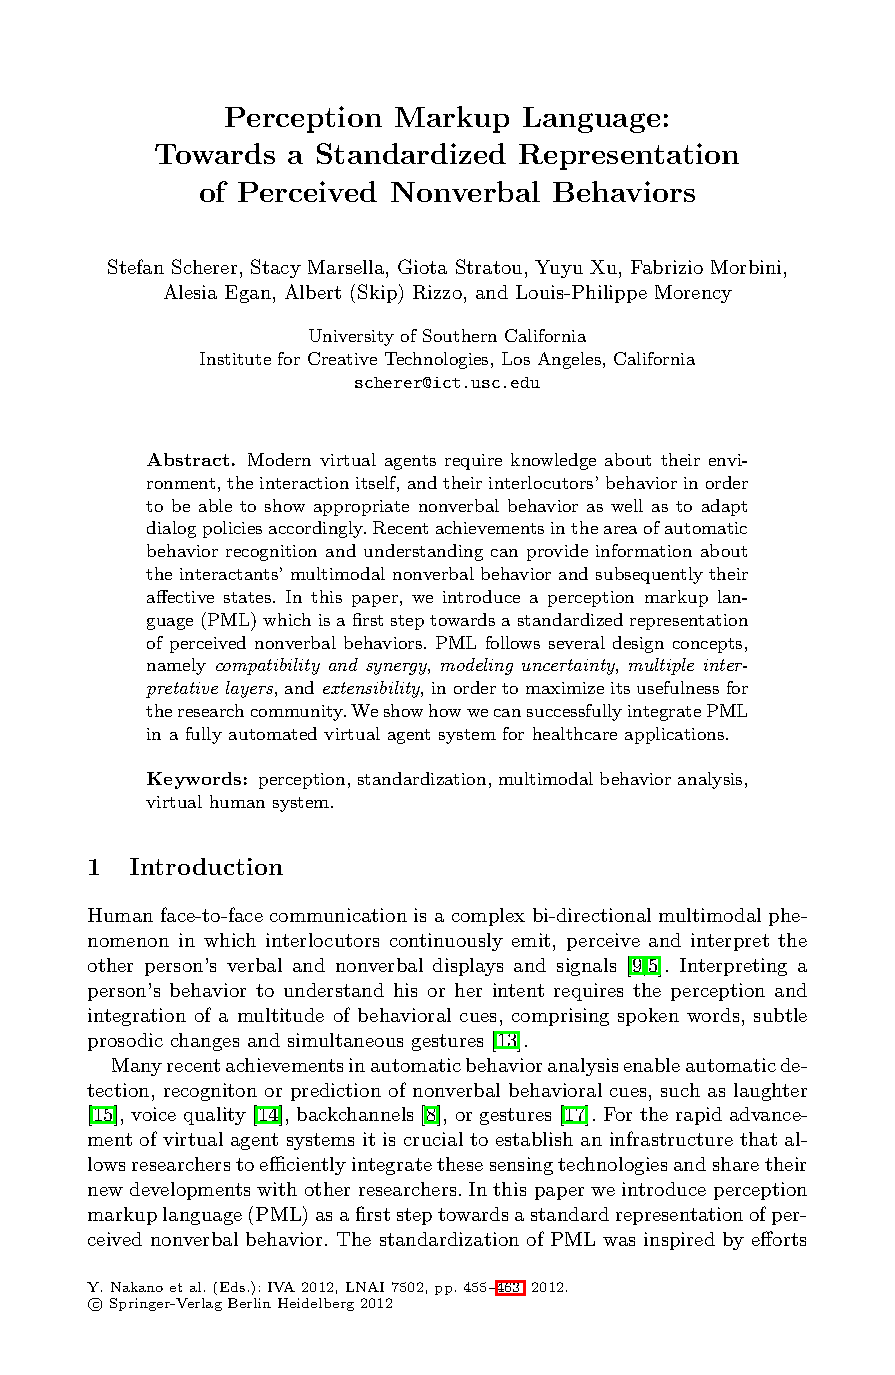
\includegraphics[keepaspectratio, width=9cm]{content/perceptionML}
  \label{pmlRole}
\end{figure}



PML doesn't specify how or when components must respond, or, which responses are possible at any given time.
  An example of a system which does be "protocol calculus" or "\pi-Calculus" which allows one to express entities which produce and consume events while going through state transitions.
  Joachim Parrow's "An Introduction to the \pi-Calculus" provides an available discussion of the topic, but, would seem to be beyond the needs of our work.\cite{bergstra2001handbook}
The goal is to standardise a way to support reusable components that enable collaboration between different teams and projects.
PML provides a language for components to communicate in, and a next step would be to build on this concept, if not the implementation, with an approach that checks the intended interactions between components is valid or even meaningful.
  Inevitably this means adopting approaches that assist with debugging and diagnosing errors when the usage of the system does not yield the intended result.
  
  
  
  
%   Compile-time check
% - no compile-time checks :(
% - might be "self-validating" because it's checked as it's built rather than as a post-build step?

% [- this standardisation allows components to exchange information in an agreed way]
%
% should discuss functional programming here?
%

  
  
% Perez

Debugging interactive software applications,\footnotemark including Virtual Humans and other Interactive AI is a complex task as errors are more difficult to produce and analyse when their preconditions are based on input caused by the user's behaviour.
\footnotetext{
  ... in comparison to non-interactive real-time systems, or, offline ones
}
Reproducing the scenario and state that caused the error can be a difficult or even impossible in a debugging context, as the application's state and timing form implicit inputs to the system.
Functional Reactive Programming (FRP) has been demonstrated to alleviate these concerns to an extent.
Time and previous states are treated as an explicit input in FRP contexts, allowing the "whole program" to operate in a "mathematically pure" method.\cite{perez2017testing}

\begin{figure}
  \caption{Illustration of FRP instaces}
  %
  % this link was used to create the image
  % https://mermaid-js.github.io/mermaid-live-editor/#/edit/eyJjb2RlIjoiXG5ncmFwaCBMUlxuXHRzdWJncmFwaCBTdGF0ZSBhdCB0aW1lIDJcblx0XHRJbnB1dDJbXCJJbnB1dFsyXTogYVwiXVxuXHRcdFNpZ25hbEZ1bmN0aW9uMltcIlNpZ25hbEZ1bmN0aW9uMjogU0YgYSBiXCJdXG5cdFx0T3V0cHV0MltcIk91dHB1dFsyXTogYlwiXVxuXHRcdElucHV0MiAtLT4gU2lnbmFsRnVuY3Rpb24yXG5cdFx0U2lnbmFsRnVuY3Rpb24yIC0tPiBPdXRwdXQyXG5cdGVuZFxuXHRzdWJncmFwaCBTdGF0ZSBhdCB0aW1lIDFcblx0XHRJbnB1dDFbXCJJbnB1dFsxXTogYVwiXVxuXHRcdFNpZ25hbEZ1bmN0aW9uMVtcIlNpZ25hbEZ1bmN0aW9uMTogU0YgYSBiXCJdXG5cdFx0T3V0cHV0MVtcIk91dHB1dFsxXTogYlwiXVxuXHRcdElucHV0MSAtLT4gU2lnbmFsRnVuY3Rpb24xXG5cdFx0U2lnbmFsRnVuY3Rpb24xIC0tPiBPdXRwdXQxXG5cdGVuZCBcblx0c3ViZ3JhcGggU3RhdGUgYXQgdGltZSAwXG5cdFx0SW5wdXQwW1wiSW5wdXRbMF06IGFcIl1cblx0XHRTaWduYWxGdW5jdGlvbjBbXCJTaWduYWxGdW5jdGlvbjA6IFNGIGEgYlwiXVxuXHRcdE91dHB1dDBbXCJPdXRwdXRbMF06IGJcIl1cblx0XHRJbnB1dDAgLS0-IFNpZ25hbEZ1bmN0aW9uMFxuXHRcdFNpZ25hbEZ1bmN0aW9uMCAtLT4gT3V0cHV0MFxuXHRlbmRcblx0U2lnbmFsRnVuY3Rpb24wID09PSBTaWduYWxGdW5jdGlvbjFcblx0U2lnbmFsRnVuY3Rpb24xID09PSBTaWduYWxGdW5jdGlvbjJcblx0IiwibWVybWFpZCI6eyJ0aGVtZSI6ImRlZmF1bHQifSwidXBkYXRlRWRpdG9yIjpmYWxzZX0
  %
  \includegraphics[keepaspectratio, width=9cm]{content/frp}
  \label{frpIllustration}
\end{figure}


At \textit{time0} Functional Reactive Programming will apply some "input" \textit{I0} to an initial instace of a \textit{signal-function}.
This will yield two values; the corresponding output \textit{O0} and the next instance of the signal function \textit{signal-function-1}.
This approach, titled Functional Reactive AnimatioN was originally developed to encode animations as declarative programs\cite{elliottHudak97fran} and has been expanded for use in interactive systems.
The innovation is the clear separation between the IO operations bringing data in and out of the simulations.
This approach allows the whole program to operate as if it was a pure functional entity\cite{perez2017testing} - when given identical streams of inputs, the program will produce identical outputs.
  This is possible since operations as minute as reading the simulation time are accounted for due to the mechanism that the simulation programmed with.
When debugging, there is the potential to record and replay sessions with greater and greater amounts of assertions, regardless of the computing resources required, until once can determine the cause of aberrant behaviour.
  Such recordings aren't limited to being used within the misbehaving device - they can be transferred to other workstations or utilised in regression testing.\cite{perez2017testing}
